\documentclass{standalone}
\usepackage{amsmath} % for \dfrac
\usepackage{../Style/Diagrams}
\tikzexternalize

\colorlet{xcol}{blue!60!black}
\colorlet{myred}{red!}
\colorlet{myblue}{blue!80!black}
\colorlet{mygreen}{green!40!black}
\colorlet{myorange}{blue}
\colorlet{mypurple}{orange}
\colorlet{mydarkred}{myred!80!black}
\colorlet{mydarkblue}{myblue!80!black}
\tikzstyle{xline}=[xcol,thick]
\tikzstyle{width}=[{Latex[length=5,width=3]}-{Latex[length=5,width=3]},thick]
\tikzset{
  traj/.style 2 args={xline,postaction={decorate},decoration={markings,
    mark=at position #1 with {\arrow{<}},
    mark=at position #2 with {\arrow{<}}}
  }
}
\def\tick#1#2{\draw[thick] (#1)++(#2:0.12) --++ (#2-180:0.24)}
\def\N{100} % number of samples


\begin{document}
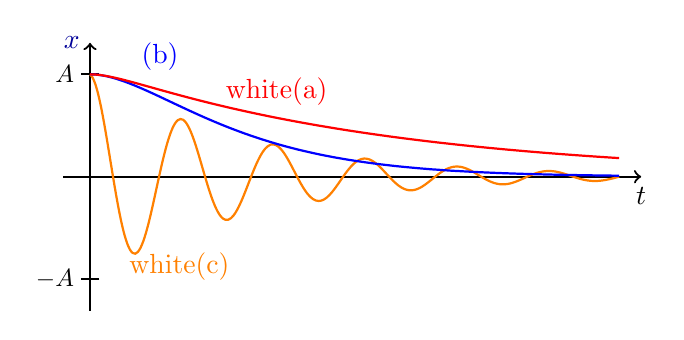
\begin{tikzpicture}
    \def\xmax{7.0} % max x axis
    \def\ymax{1.7} % max y axis
    \def\A{1.3}
    \def\om{(6.5/(0.94*\xmax))} % natural omega_0
    \def\Za{0.50} % zeta underdamped 1
    \def\Zb{0.95} % zeta underdamped 2
    \def\Zc{1.00} % zeta critically damped
    \def\Zd{2.00} % zeta overdamped
    \def\Ga{(\Za*\om)} % gamma underdamped 1
    \def\Gb{(\Zb*\om)} % gamma underdamped 2
    \def\Gc{\om}       % gamma critically damped
    \def\Gd{(\Zd*\om)} % gamma overdamped
    \def\Wa{(\om*sqrt(1-\Za*\Za)}  % omega underdamped 1
    \def\Wb{(\om*sqrt(1-\Zb*\Zb)}  % omega underdamped 2
    \def\Wd{(\om*sqrt(\Zd*\Zd-1))} % omega overdamped
    
    % AXIS
    \draw[->,thick] (0,-\ymax) -- (0,\ymax) node[left,xcol] {$x$};
    \draw[->,thick] (-0.2*\ymax,0) -- (\xmax,0) node[below] {$t$};
    \tick{0,\A}{0} node[left=-1,scale=0.9] {$A$};
    \tick{0,-\A}{0} node[left=-1,scale=0.9] {$-A$};
    
    % PLOT
    \draw[xline,mypurple,samples=100+\N,smooth,variable=\t,domain=0:0.96*\xmax]
      plot(\t,{\A*exp(-\Ga*\t)*cos(360*\Wa*\t)});
    \draw[xline,myorange,samples=\N,smooth,variable=\t,domain=0:0.96*\xmax]
      plot(\t,{\A*(1+\Gc*\t)*exp(-\Gc*\t)});
    \draw[xline,myred,samples=\N,smooth,variable=\t,domain=0:0.96*\xmax]
      plot(\t,{\A/2*( (1+\Gd/\Wd)*exp((\Wd-\Gd)*\t) + (1-\Gd/\Wd)*exp(-(\Wd+\Gd)*\t))});
    %\node[above=4] at (0.15*\xmax,{\A*exp(-0.15*\xmax/\T)}) {$e^{-\frac{b}{2m}t}$};
    
    % NODES
    \node[below,mypurple]   at ({1.15*\om},-0.65*\A) {\contour{white}{(c)}};
    \node[above,myorange]   at ({0.90*\om}, 0.94*\A) {(b)};
    \node[above,myred]      at ({2.40*\om}, 0.60*\A) {\contour{white}{(a)}};
    
  \end{tikzpicture}
\end{document}